\documentclass[12pt]{article}
\usepackage{amsmath}
\usepackage{amsfonts}
\usepackage{hyperref}
\usepackage{tikz} 
\usetikzlibrary {shapes.misc} 
\usepackage[bottom]{footmisc}
\usepackage[left = 1in, right = 1in, top = 1in, bottom = 1in]{geometry}


\title{Cellular Automaton on Hanoi Graphs}
\author{Geethan Pfeifer}
%\date{}

\newcommand{\abs}[1]{\left\lvert #1 \right\rvert}
\newcommand{\pd}[2]{\frac{\partial #1}{\partial #2}}
\newcommand{\df}[2]{\frac{\mathrm{d} #1}{\mathrm{d} #2}}

\renewcommand\Re{\operatorname{Re}}
\renewcommand\Im{\operatorname{Im}}


\begin{document}
	
	\maketitle
	
	\section{Introduction}
	This document informally describes cellular automaton on Hanoi Graphs, which resemble Sierpinski Triangles, and also a basic implementation in \href{https://golly.sourceforge.io/}{Golly}.
	\section{Hanoi Graphs}
	Read \url{https://mathworld.wolfram.com/HanoiGraph.html} for an introduction to Hanoi Graphs.
	\section{Structure of Hanoi Graphs}
	Every Hanoi graph has 3 vertices of degree 2 (denote these vertices as \textit{corner} vertices), with every other vertex having degree 3 (denote these vertices as \textit{inner} vertices.)\footnote{These are not standard definitions, I'm just defining them as such for convenience.}\\
	Each inner vertex is part of a 3-clique and a 2-clique.
	\section{Neighbourhood}\label{nei}
	Consider a Hanoi Graph $H_n$ as you would typically on a plane.\\
	For each inner vertex $u$, consider the vertex it forms a 2-clique with as $\operatorname{P}(u)$. Consider the vertices it forms a 3-clique with as $\operatorname{N}_1(u)$, $\operatorname{N}_2(u)$, with $\operatorname{N}_1(u)$ being clockwise to $u$ and $\operatorname{N}_2(u)$ being counterclockwise to $u$.\\
	Define the neighbourhood of $u$ as the tuple $(u, \operatorname{P}(u), \operatorname{N}_1(u),\operatorname{N}_2(u))$. 
	\pagebreak
	\subsection{Example}\label{ex1}
	For example, consider $H_2$ below, with labelled inner vertex $u$, and labelled $\operatorname{P}(u)$, $\operatorname{N}_1(u)$, and $\operatorname{N}_2(u)$.
% https://tex.stackexchange.com/q/270543
\begin{center}
	\begin{tikzpicture}[minimum size=1.5cm]
		\node[shape=circle, draw=black] (A) at (0,0) {};
		\node[shape=circle, draw=black] (B) at (-1.5,-2.598) {};
		\node[shape=circle, draw=black] (C) at (1.5,-2.598) {$\operatorname{P}(u)$};
		\node[shape=circle, draw=black] (D) at (-3,-5.196) {};
		\node[shape=circle, draw=black] (E) at (-4.5,-7.794) {};
		\node[shape=circle, draw=black] (F) at (-1.5,-7.794) {};
		\node[shape=circle, draw=black] (G) at (3,-5.196) {u};
		\node[shape=circle, draw=black] (H) at (1.5,-7.794) {$\operatorname{N}_2(u)$};
		\node[shape=circle, draw=black] (I) at (4.5,-7.794) {$\operatorname{N}_1(u)$};
		
		\path[-](A) edge (B);
		\path[-](A) edge (C);
		\path[-](C) edge (B);
		\path[-](D) edge (E);
		\path[-](E) edge (F);
		\path[-](F) edge (D);
		\path[-](G) edge (H);
		\path[-](H) edge (I);
		\path[-](I) edge (G);
		\path[-](B) edge (D);
		\path[-](F) edge (H);
		\path[-](C) edge (G);		
		
	\end{tikzpicture}
\end{center}	
	\subsection{Note}
		On a Hanoi graph, for a inner vertex $u$ with $\operatorname{P}(u)$, $\operatorname{N}_1(u)$, and $\operatorname{N}_2(u)$ also inner vertices, $\operatorname{P}(\operatorname{P}(u)) = u$, $\operatorname{N}_1(\operatorname{N}_1(\operatorname{N}_1(u)))=u$, and $\operatorname{N}_2(\operatorname{N}_2(\operatorname{N}_2(u)))=u$.
	\section{Cellular Automaton}
		Take a Hanoi Graph $H_n = (V, E)$, with inner vertices $I$.\\
		Let $Q$ be the set of states.\\
		Define a transition function $\delta: Q^4 \rightarrow Q$.\\\\
		Define $\operatorname{CA}_0(u) : V \rightarrow Q$.\\
		For $t > 0$, define:
		$$\operatorname{CA}_t : V \rightarrow Q,$$$$\operatorname{CA}_t(u) = \begin{cases}
			\delta(\operatorname{CA}_{t-1}(u),\operatorname{CA}_{t-1}(\operatorname{P}(u)),\operatorname{CA}_{t-1}(\operatorname{N_1}(u)),\operatorname{CA}_{t-1}(\operatorname{N_2}(u))), & u \in I\\
			\operatorname{undefined}, & u \notin I
		
		\end{cases} $$
		For convenience, we can define $CA_t(u) = CA_0(u), u \notin I$, but other options are possible.\\\\
		Concisely, the state of an inner vertex $u$ depends on the states of its neighbours and itself in the previous generation, and the state of corner vertices is undefined.
	\section{Elementary Automaton}\label{ela}
		Take $Q = \{0,1\}$. Clearly, there are $2^{2^4} = 65536$ possible transition functions.\\
		We can number them with $16$-bit integers, with the $m$-th bit of $n$ being the value of $\delta_n(m_0, m_1, m_2, m_3)$, where $m_3m_2m_1m_0$ is the binary representation of $m$.\\
		Call $\delta_n$ \texttt{Sierpinski n}\footnote{Perhaps \texttt{Hanoi n} is a better name, but I already named it \texttt{Sierpinski n} in my Golly implementation.}
		\subsection{Example}
		For example, take \texttt{Sierpinski 49980}.\\
		The binary representation of $49980$ is $1100001100111100_2$. \\This is the transition table:
% https://www.overleaf.com/learn/latex/Tables
		\begin{center}
		\begin{tabular}{ c|||c|c|c|c||c }
			$m$ & $\operatorname{CA}_{t-1}(u)$ & $\operatorname{CA}_{t-1}(\operatorname{P}(u))$ & $\operatorname{CA}_{t-1}(\operatorname{N_1}(u))$ & $\operatorname{CA}_{t-1}(\operatorname{N_2}(u))$ & $\operatorname{CA}_{t}(u)$\\
			\hline
			0 & 0 & 0 & 0 & 0 & 0\\
			1 & 1 & 0 & 0 & 0 & 0\\
			2 & 0 & 1 & 0 & 0 & 1\\
			3 & 1 & 1 & 0 & 0 & 1\\
			4 & 0 & 0 & 1 & 0 & 1\\
			5 & 1 & 0 & 1 & 0 & 1\\
			6 & 0 & 1 & 1 & 0 & 0\\
			7 & 1 & 1 & 1 & 0 & 0\\
			8 & 0 & 0 & 0 & 1 & 1\\
			9 & 1 & 0 & 0 & 1 & 1\\
			10 & 0 & 1 & 0 & 1 & 0\\
			11 & 1 & 1 & 0 & 1 & 0\\
			12 & 0 & 0 & 1 & 1 & 0\\
			13 & 1 & 0 & 1 & 1 & 0\\
			14 & 0 & 1 & 1 & 1 & 1\\
			15 & 1 & 1 & 1 & 1 & 1\\
			
			
			
						\end{tabular}
		\end{center}
	(This rule updates to the XOR sum of the neighbours of a vertex.)
	\pagebreak
	\section{Golly}
	\subsection{Representation on a 2-D grid}
	If you ``skew'' the planar representation of a Hanoi Graph slightly it fits nicely on a 2D grid. For example, we can ``skew'' the graph in \ref{ex1} as such:
\begin{center}
	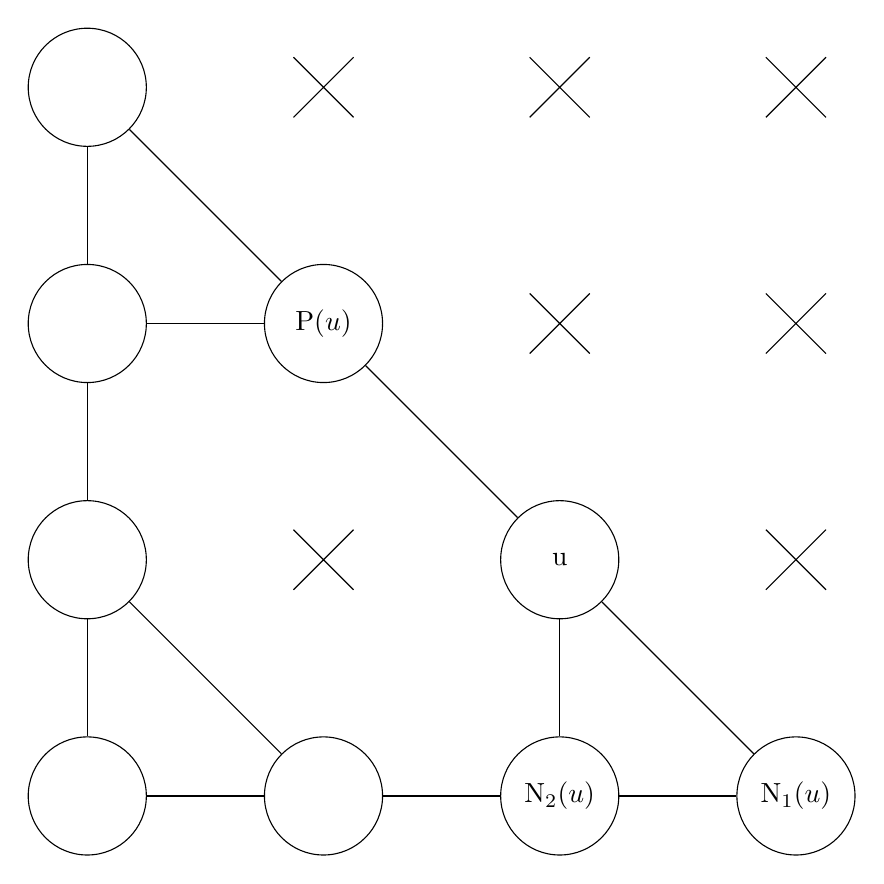
\begin{tikzpicture}%[minimum size=1.5cm]
		\node[shape=circle, draw=black, minimum size = 1.5cm] (A) at (0,0) {};
		\node[shape=circle, draw=black, minimum size = 1.5cm] (B) at (0, -3) {};
		\node[shape=circle, draw=black, minimum size = 1.5cm] (C) at (3, -3) {$\operatorname{P}(u)$};
		\node[shape=circle, draw=black, minimum size = 1.5cm] (D) at (0,-6) {};
		\node[shape=circle, draw=black, minimum size = 1.5cm] (E) at (0,-9) {};
		\node[shape=circle, draw=black, minimum size = 1.5cm] (F) at (3,-9) {};
		\node[shape=circle, draw=black, minimum size = 1.5cm] (G) at (6, -6) {u};
		\node[shape=circle, draw=black, minimum size = 1.5cm] (H) at (6, -9) {$\operatorname{N}_2(u)$};
		\node[shape=circle, draw=black, minimum size = 1.5cm] (I) at (9,-9) {$\operatorname{N}_1(u)$};
		
		\node[shape = cross out, draw=black, minimum size = 0.75cm] (E1) at (3, 0) {};
		\node[shape = cross out, draw=black, minimum size = 0.75cm] (E2) at (6, 0) {};
		\node[shape = cross out, draw=black, minimum size = 0.75cm] (E3) at (9, 0) {};
		\node[shape = cross out, draw=black, minimum size = 0.75cm] (E4) at (6, -3) {};
		\node[shape = cross out, draw=black, minimum size = 0.75cm] (E5) at (9, -3) {};
		\node[shape = cross out, draw=black, minimum size = 0.75cm] (E6) at (3, -6) {};
		\node[shape = cross out, draw=black, minimum size = 0.75cm] (E7) at (9, -6) {};
		
		\path[-](A) edge (B);
		\path[-](A) edge (C);
		\path[-](C) edge (B);
		\path[-](D) edge (E);
		\path[-](E) edge (F);
		\path[-](F) edge (D);
		\path[-](G) edge (H);
		\path[-](H) edge (I);
		\path[-](I) edge (G);
		\path[-](B) edge (D);
		\path[-](F) edge (H);
		\path[-](C) edge (G);		
		
	\end{tikzpicture}
\end{center}	
Each cross represents an empty square.
\subsection{Advantages of this representation}
The neighbourhood of an inner vertex $u$ as defined in \ref{nei} (and their states) can be determined solely by the Moore neighbourhood of $u$ on the 2D grid, meaning that we can create Golly rules for it.\footnote{I was shocked to discover that there are very few neighbourhoods supported by Golly! I initially planned to use a different representation, but that representation wouldn't be possible with a neighbourhood supported by Golly.}\\
Also, this representation of the Hanoi Graph can be easily generated by \texttt{Wolfram 60}.
\subsection{Generating golly rules}
\href{https://github.com/GeethanPfeifer/sierpinski/blob/main/golly/sierpinskirulegen.cpp}{sierpinskirulegen} generates a Golly rule corresponding to a specified Sierpinski rule. In the rule, state \texttt{0} corresponds to an empty square, and states \texttt{1} and \texttt{2} correspond to states $0$ and $1$ as per \ref{ela} respectively.

\section{Future work}
\begin{itemize}
	\item Develop an ``infinite Hanoi graph'' such that all vertices are inner.
	\item Develop analogues of tori such that all vertices are inner.
	\item Create a custom program for cellular automaton on fractal patterns--Golly is quite limited.
	\item Develop the concept of a ``direction''. (How would spaceships work with these cellular automaton? Are they even possible?)

	
\end{itemize}\pagebreak
\begin{thebibliography}{9}
	\bibitem{wr1}
	Weisstein, Eric W. ``Hanoi Graph.'' From \textit{MathWorld}--A Wolfram Web Resource.\\ \url{https://mathworld.wolfram.com/HanoiGraph.html}
	
	\bibitem{wr2}
	Weisstein, Eric W. ``Elementary Cellular Automaton.'' From \textit{MathWorld}--A Wolfram Web Resource. \\\url{https://mathworld.wolfram.com/ElementaryCellularAutomaton.html}
	
	\bibitem{cl1}
	LifeWiki. ``Moore neighbourhood.'' Retrieved on January 10, 2025.\\ \url{https://conwaylife.com/wiki/Moore_neighbourhood}
	
	\bibitem{cl2}
	LifeWiki. ``Tutorials/Creating custom rules''. Retrieved on January 10, 2025.\\
	\url{https://conwaylife.com/wiki/Tutorials/Creating_custom_rules}
\end{thebibliography}
\end{document}